%%% Local Variables:
%%% TeX-command-extra-options: "-shell-escape"
%%% End:

\documentclass{beamer}

\usepackage[utf8]{inputenc}
\usetheme{Madrid}
\usecolortheme{beaver}
\usepackage{minted}
\usepackage{graphicx}
\graphicspath{{./images/}}

\newminted{apache}{fontsize=\scriptsize, 
  numbersep=8pt,
  gobble=4,
  frame=lines,
  fontfamily=courier,
  fontsize=\small,
  bgcolor=bg,
  framesep=3mm} 

\newminted{docker}{fontsize=\scriptsize, 
  numbersep=8pt,
  gobble=4,
  frame=lines,
  fontfamily=courier,
  fontsize=\small,
  bgcolor=bg,
  framesep=3mm
} 

\newminted{yaml}{fontsize=\scriptsize, 
  numbersep=8pt,
  gobble=4,
  frame=lines,
  fontfamily=courier,
  fontsize=\small,
  bgcolor=bg,
  framesep=3mm} 

\newminted{bash}{fontsize=\scriptsize, 
  numbersep=8pt,
  gobble=4,
  frame=lines,
  fontfamily=courier,
  fontsize=\small,
  bgcolor=bg,
  framesep=3mm} 

% Information to be included in the title page:
\title{Openshift}
\subtitle{Introduction to the Side Car}
\author{Spike Spiegel}
\institute{Cowboy Bebop}
\date{Auguste 2018}

\logo{
\includegraphics[height=0.7cm]{2753308_0.jpg}}

\begin{document}

\frame{\titlepage}

\definecolor{bg}{rgb}{0.95,0.95,0.95}

\begin{frame}[fragile]
  \frametitle{Schema}
\begin{figure}[ht]
  \caption{schema of a Side Car}
  \centering
  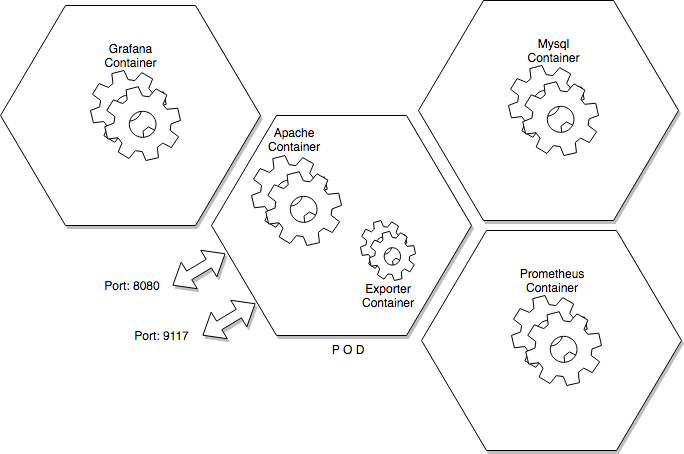
\includegraphics[scale=0.6]{SidecarDiagram.png}
  \label{fig:SidecarDiagram}
\end{figure}
\end{frame}

\begin{frame}[fragile]
  \frametitle{Apache status}
  Module to enable the output statistic of \emph{Apache}.
  
  \begin{figure}
    \begin{apachecode}
      <Location /server-status>
      SetHandler server-status
      Order deny,allow
      Allow from all
      </Location> ExtendedStatus On>
    \end{apachecode}
    \caption{status.conf}
    
    This module will be copied in the \emph{/etc/apache2/mods-enabled/} directory.
  \end{figure}
\end{frame}

\begin{frame}[fragile]
  \frametitle{Dockerfile}
  The \emph{Dockerfile} include the copy of the \emph{Apache} module.\\
  Important to add the switching between \textit{root} and \textit{1001} user
  \begin{figure}
    \begin{dockercode}
      FROM ubuntu:latest
      USER root
      ...
      RUN a2enmod status
      COPY status.conf /etc/apache2/mods-enabled/
      EXPOSE 8080
      USER 1001
      CMD ["/usr/sbin/apache2ctl", "-DFOREGROUND"]
    \end{dockercode}
    \caption{Dockerfile}
  \end{figure}
  
\end{frame}

\begin{frame}[fragile]
  \frametitle{Secret Access}
  And because the credential of \emph{GITLAB}
  \begin{figure}
    \begin{yamlcode}
      apiVersion: v1
      kind: Secret
      metadata:
      name: github-secret
      namespace: sidecar
      type: kubernetes.io/basic-auth
      data:
      username: c3Bpa2U=
      password: dmFsZW50aW5l
    \end{yamlcode}
    \caption{gitlab-secret.yaml}
  \end{figure}
\end{frame}

\begin{frame}[fragile]
  \frametitle{Secret Access}
  The \emph{username} and \emph{password} are coded with this method and we load the new \emph{secret}
  \begin{bashcode}
    $ echo -n 'spike' | base64
    c3Bpa2U=
    $ echo -n 'valentine' | base64
    dmFsZW50aW5l
    $ oc create -f gitlab-secret.yaml
  \end{bashcode}
\end{frame}

\begin{frame}[fragile]
  \frametitle{New Project}
  It's time to create our new project \emph{sidecar}, similar to a namespace 
  \begin{bashcode}
    $ oc new-project sidecar \
    --display-name='Side Car Project' \
    --description='Side Car Project'
  \end{bashcode}
\end{frame}

\begin{frame}[fragile]
  \frametitle{New Build}
  We build our new image \emph{faye}, linked to the new secret and we restart the build process
  \begin{bashcode}
    $ oc new-build http://192.168.0.8:8880/spike/faye.git \
    --name faye
    $ oc set build-secret --source bc/faye github-secret
    $ oc start-build faye
  \end{bashcode}
\end{frame}

\begin{frame}[fragile]
  \frametitle{New Build more friendly}
  A other solution concists to build the new image with a same command line
  \begin{bashcode}
    $ oc new-build http://192.168.0.8:8880/spike/faye.git \
    --source-secret github-secret \
    --name faye
  \end{bashcode}
\end{frame}

\begin{frame}[fragile]
  \frametitle{New Application}
  It's time to create our application based on the new image \emph{faye}
  \begin{bashcode}
    $ oc new-app faye \
    --name fayeapp
    $ oc status
    $ oc expose service faye
    $ oc get pod
    $ oc get all name --selector app=cdnselect
  \end{bashcode}
\end{frame}

\begin{frame}[fragile]
  \frametitle{Export}
  We export the new application to have a base for the next process\\
  The final application will be based on the export.
  \begin{bashcode}
    $ oc get --export is,bc,dc,svc -o yaml > export.yaml
  \end{bashcode}
\end{frame}

\begin{frame}[fragile]
  \frametitle{Item To Modify}
  4 parts will be modified to adapted to our application
  \begin{itemize}
  \item ImageStream
  \item BuildConfig
  \item DeploymentConfig
  \item Service
  \end{itemize}
\end{frame}

\begin{frame}[fragile]
  \frametitle{ImageStream}
  We delete resourceVersion, selfLink and uid. In status, we keep dockerImageRepository (set to ””)
  \begin{yamlcode}
    status:                                                                                                           
    dockerImageRepository: "" 
  \end{yamlcode}
\end{frame}

\begin{frame}[fragile]
  \frametitle{BuildConfig}
  We delete resourceVersion, selfLink and uid. We delete in spec.triggers.imageChange lastTriggeredImageID
  \begin{yamlcode}
    triggers:                                                                                                       
    - github:                                                                                                       
        secret: -sFpqvH1ZtjwSybAZkRI                                                                                
      type: GitHub                                                                                                  
    - generic:                                                                                                      
      secret: CSGghgKGL2kTVIr8l5Nc                                                                                
      type: Generic                                                                                                 
    - type: ConfigChange                                                                                            
    - imageChange:                                                                                                  
      type: ImageChange
  \end{yamlcode}
\end{frame}

\begin{frame}[fragile]
  \frametitle{DeploymentConfig}
  We replace spec.template.spec.containers.image by faye in the first container and we add in spec.template.spec.container
  \begin{yamlcode}
    spec:
      containers: 
      - name: apache-exporter
      image: previousnext/apache-exporter
      command: [ "apache_exporter", "-scrape_uri", \
      "http://127.0.0.1:8080/server-status/?auto" ]
      ports:
      - containerPort: 9117
      ...
  \end{yamlcode}
\end{frame}

\begin{frame}[fragile]
  \frametitle{Service}
  We add in spec.ports
  \begin{yamlcode}
    spec:                                                                                                             
      clusterIP: 172.30.7.204                                                                                         
      ports:                                                                                                          
      - name: 8080-tcp                                                                                                
      port: 8080                                                                                                    
      protocol: TCP                                                                                                 
      targetPort: 8080 
      - name: 9117-tcp
      port: 9117
      protocol: TCP
      targetPort: 9117
  \end{yamlcode}
  The port related to our \emph{exporter apache}
\end{frame}

\begin{frame}[fragile]
  \frametitle{Finally}
  Finally we create our new application from this \emph{yaml} file
  \begin{bashcode}
    $ oc create -f export.yaml
  \end{bashcode}
  Et voila...
\end{frame}

\end{document}